%\documentclass[10pt,a4paper]{article}

% headsepline: Linie am oberen Blattrand unterhalb der Seitennummer
% bibtotoc: Aufnahme des Literaturverzeichnisses ins Inhaltsverzeichnis
\documentclass[a4paper,headsepline,bibtotoc]{scrreprt}
\usepackage[utf8]{inputenc}
\usepackage{amsmath}
\usepackage{amsfonts}
\usepackage{amssymb}
% Einstellungen bez. des 'scrreprt'-Stils
% Caption Schriftstil und -Groesse
\renewcommand{\capfont}{\footnotesize}
\renewcommand{\caplabelfont}{\footnotesize\bfseries}
\typearea{15}  %Einstellung des Verh�ltnisses Gr��e des Textes zur Papiergr��e
% Sprache
\usepackage[german,english]{babel}
\selectlanguage{german}
\setlength{\parindent}{0pt}


\usepackage{pgfplots}
\usepackage{tikz}
\usepackage{caption}
\usepackage{subcaption}
\usepgfplotslibrary{external}
\usepackage{pdfpages}
\usepackage{lipsum}  




\addto\extrasgerman{\renewcommand{\figurename}{Abb.}}
\addto\extrasgerman{\renewcommand{\tablename}{Tab.}}

% Bilder
\usepackage[rflt]{floatflt}
\usepackage{epsfig,wrapfig}

% Programmablaufplaene (Struktogramme, Nassi-Schneidermann-Diagramme)
% Dieses Paket ist nicht standardm��ig im CIP-Pool installiert
% \usepackage{nassi}

% Mathematische Symbole
\usepackage{amsmath,amssymb}

% Tabellen
\usepackage{longtable,lscape}
\usepackage{multirow}
\usepackage{tabularx}

% Kopfzeilen
\usepackage{fancyheadings}
\pagestyle{plain}
\renewcommand{\chaptermark}[1]{\markboth{#1}{}}
\renewcommand{\sectionmark}[1]{\markboth{\thesection\ #1}{}}
\lhead[\fancyplain{}{\sl\leftmark}]%
      {\fancyplain{}{\sl\leftmark}}
\rhead[\fancyplain{}{\sl\thepage}]%
      {\fancyplain{}{\sl\thepage}}
\cfoot{}

% Aufgabenstellung
\usepackage{iagkopf}

\graphicspath{ {./images/} }

% Listenerscheinung
\setlength{\itemsep}{0ex}
\setlength{\parsep}{0ex}
\setlength{\parskip}{2mm}


\begin{document}
\sloppy

% Seitennumerierung bis zum Beginn der Einleitung auf kleine roemische Zahlen setzen
\pagenumbering{roman}

% neue Befehle
%\newcommand{\file}[1]{{\sffamily\slshape #1}}
\newcommand{\file}[1]{\mdseries\textsl{\textsf{#1}}}
\newcommand{\sbr}[1]{\texttt{#1}}
\newcommand{\var}[1]{\mdseries\textsl{\texttt{#1}}}
\newcommand{\cmd}[1]{\uppercase{\texttt{#1}}}

% Titelseite
\title{Implementation and Validation of Finite Rate Chemical Kinetics in FLEXI}

\author{Master Thesis \\
        by \\
        Sinan Felix Klein}

\publishers{conducted at the \\
            Institute of Aerodynamics and Gas Dynamics \\
            University of Stuttgart.
            \\[5ex]
            Stuttgart, April 2025}

\date{}


\selectlanguage{english}

\maketitle

\newpage
\thispagestyle{empty} 
\section*{}
\newpage

% Aufgabenstellung einbinden
\addcontentsline{toc}{chapter}{Assignment}
\pagestyle{plain}
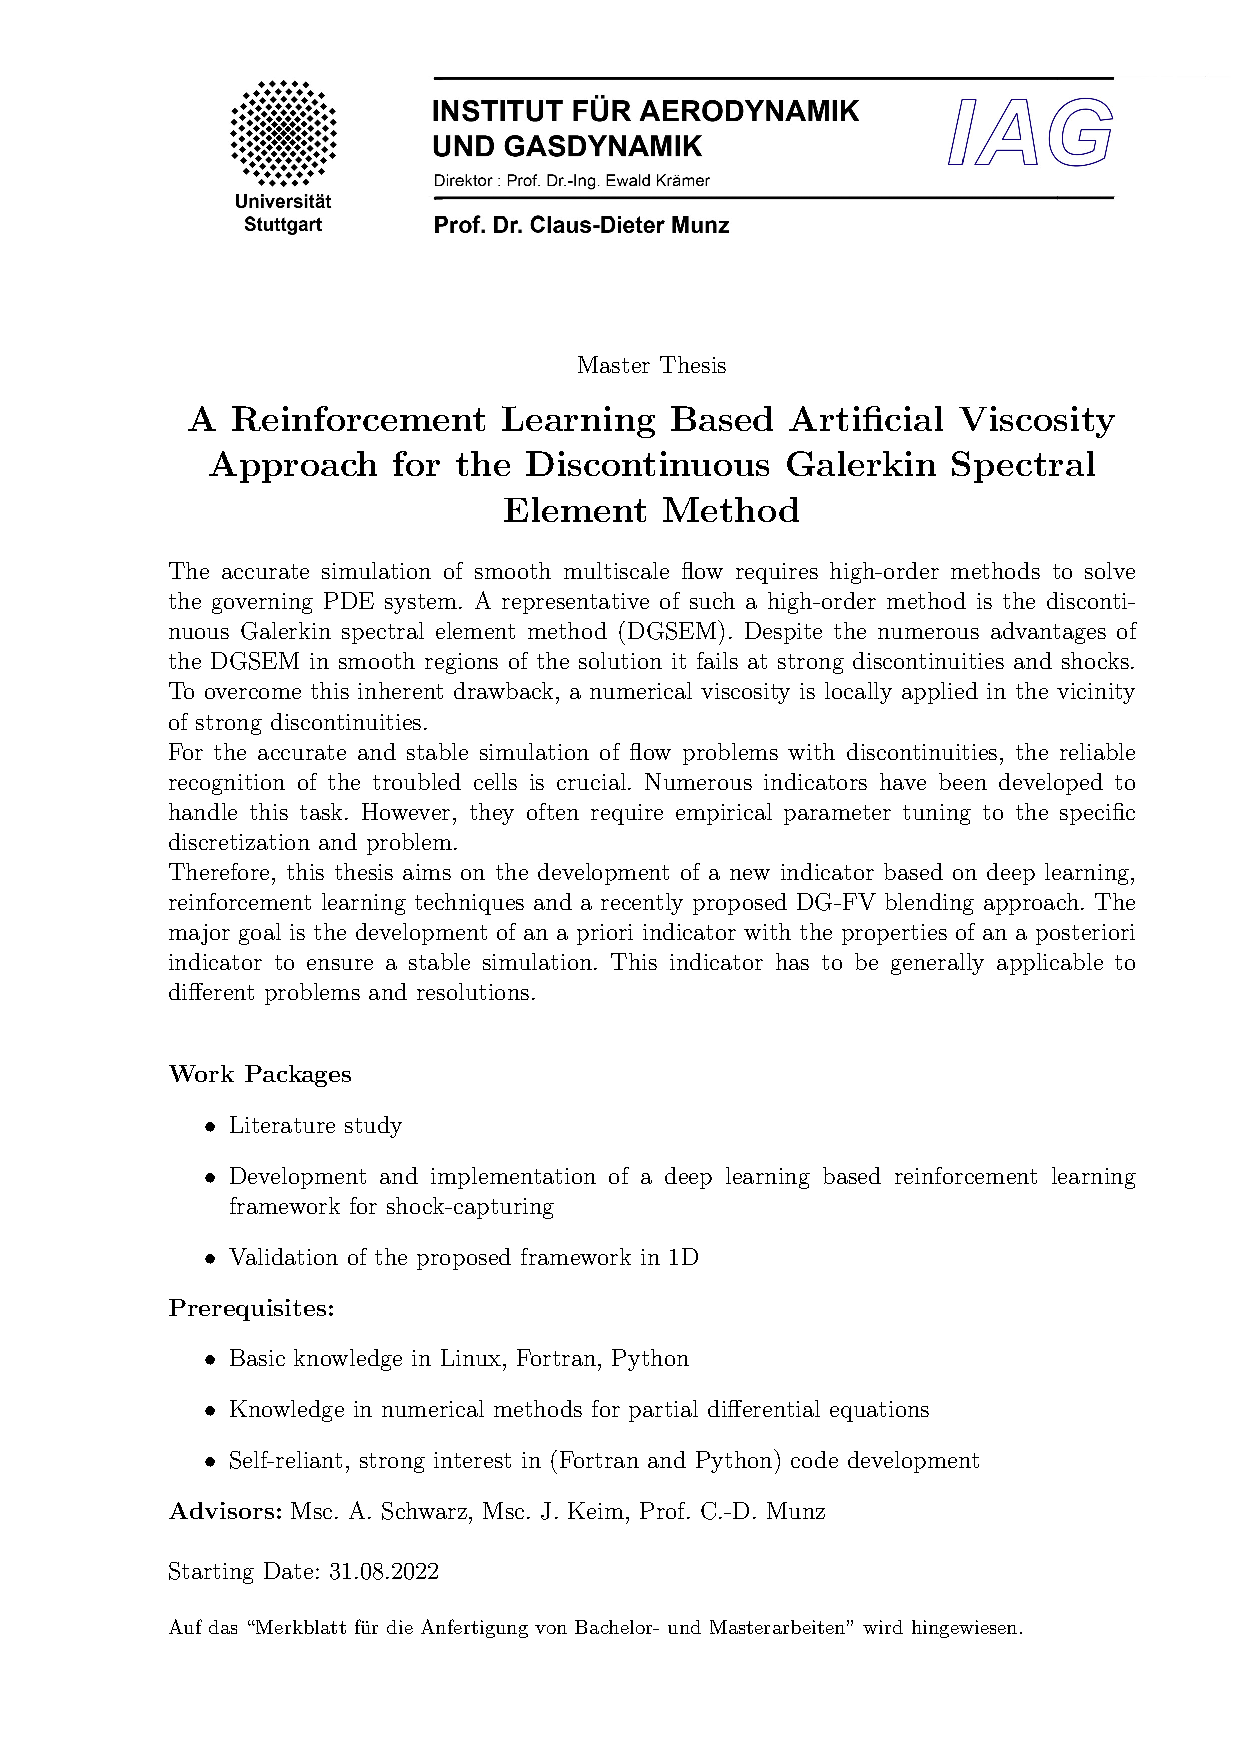
\includepdf[pages=1]{aufgabenstellung_rlindi_msc}


\newpage
\thispagestyle{empty} 
\section*{}
\newpage

% �bersicht
\newpage
\chapter*{Erkl\"arung}
Hiermit versichere ich, dass ich diese Masterarbeit selbstständig mit Unterstützung der Betreuer angefertigt und keine
anderen als die angegebenen Quellen und Hilfsmittel verwendet habe.
Die Arbeit oder wesentliche Bestandteile davon sind weder an dieser noch an einer anderen Bildungseinrichtung bereits zur Erlangung eines Abschlusses eingereicht worden.
Ich erkläre weiterhin, bei der Erstellung der Arbeit die einschlägigen Bestimmungen zum Urheberschutz fremder Beiträge entsprechend den Regeln guter wissenschaftlicher Praxis1 eingehalten zu haben. Soweit meine Arbeit fremde Beiträge (z.B. Bilder, Zeichnungen, Textpassagen etc.) enthält, habe ich diese Beiträge als solche gekennzeichnet (Zitat, Quellenangabe) und eventuell erforderlich gewordene Zustimmungen der Urheber zur Nutzung dieser Beiträge in meiner Arbeit eingeholt. Mir ist bekannt, dass ich im Falle einer schuldhaften Verletzung dieser Pflichten die daraus entstehenden Konsequenzen zu tragen habe. 
\\
\\
\\

………………………………………\\
Ort, Datum, Unterschrift



\newpage
\thispagestyle{empty} 
\section*{}
\newpage

\addcontentsline{toc}{chapter}{Abstract}
\pagestyle{plain}
\chapter*{Abstract}

	

\newpage
\thispagestyle{empty} 
\section*{}
\newpage

% Nomenklatur
\addcontentsline{toc}{chapter}{Nomenclature}
\pagestyle{plain}
\chapter*{Nomenclature}
\begin{tabular}{lll}
    \vspace{1mm}
   $a$              & [-]             & 
Wave speed\\
   \vspace{1mm}
   $a^{l-1}$              & [-]             & Input into MLP layer l\\  
  \vspace{1mm}
      $A,a$              & [-]             & Action\\ 
    \vspace{1mm}
     $A$              & [-]             & Amplitude of SineWave test case \\
    \vspace{1mm}
     $b^l$              & [-]             & Bias of MLP layer l\\  
     $\underline{\underline{B}}$              & [-]             & Boundary matrix\\   
    \vspace{1mm}
    $c$              & [-]             & Constant for target clipping\\
      \vspace{1mm}
    $c$              & [-]             & Crashed flag\\
    \vspace{1mm}
   $c_{act}$              & [-]             & Diminishing factor for exploring with random action\\
    \vspace{1mm}
   $c_1,c_2,c_3$              & [-]             & Reward hyperparameters\\ 
    \vspace{1mm}
       $C$              & [-]             & Loss function\\          	\vspace{1mm}
       $d$              & [-]             & Done flag\\    	
       \vspace{1mm}
       $\underline{\underline{D}}$              & [-]             & Derivative matrix\\    
   \vspace{1mm} 
  $e$        & [$\text{m}^2\text{s}^{-2}$]            & Total energy per unity volume \\
  \vspace{1mm}
     $E, \tilde{E}_{ref}, \tilde{E}^{sub}$              & [-]             & Physical Element, Reference Element, Subelement \\
   \vspace{1mm}
     $f$              & [-]             & Convective flux \\
     \vspace{1mm}
     $f$              & [-]             & Frequency of SineWave test case \\
     \vspace{1mm}   
    $f^\#$              & [-]             & Two-point entropy preserving flux\\  
   \vspace{1mm}
      $f_{act}$              & [-]             & Activation function\\     
   \vspace{1mm}
   $\underline{F}_{Surf},\underline{F}_{Vol}$              & [-]             & Surface and volume Integral\\  
   \vspace{1mm}
      $g$              & [-]             & 
Numerical flux\\
   \vspace{1mm}
   $G$              & [-]             & Return\\ 
   \vspace{1mm}      
  $h$              & [$\text{m}^2\text{s}^{-2}\text{kg}^{-1}$]             & Specific enthalpy \\  
    \vspace{1mm}
   $I_{jump}$              & [-]             & Jump indicator function\\ 
       \vspace{1mm}
   $I_{MOOD}$              & [-]             & MOOD indicator function\\      
     \vspace{1mm}
   $I_{sanity}$              & [-]             & Sanity check function\\    
  \vspace{1mm}
   $J$              & [-]             & Expected return\\ 
   \vspace{1mm}
   $J$              & [-]             & Jacobian for mapping to reference space\\    
   \vspace{1mm}
   $J_{ele},J_{stc},J_{tresh}$              & [-]             & Summed up jumps in element/stencil/threshold \\ 
  \vspace{1mm}
   $j$              & [-]             & Initial pressure jump \\
   \vspace{1mm}
   $K^l$              & [-]             & Number of neurons in previous layer l-1\\         
   \vspace{1mm}
   $L,l$              & [-]             & Number of layers inside MLP, layer of MLP\\    
   \vspace{1mm}
   $l$              & [-]            & Lagrange function \\
   \vspace{1mm}
   $M^l$              & [-]             & Number of neurons in layer l\\         
   \vspace{1mm}
   $\underline{\underline{M}}$              & [-]             & Mass matrix\\
      \vspace{1mm}
          $n$              & [-]             & 
Normal vector at element boundary\\   
\vspace{1mm}
\end{tabular}

\begin{tabular}{lll}
   \vspace{1mm}
   $n_{B}$              & [-]             & Number sample tupels in minibatches\\
   \vspace{1mm}
      $n_{epochs}$              & [-]             & Number of epochs\\
    \vspace{1mm}
   $n_{updates}$              & [-]             & Number of minibatches\\
       \vspace{1mm}
     $N$              & [-]             & Order of the DG polynomial\\     
   \vspace{1mm}
   $N_{delay}$              & [-]             & Frequency of policy and target updates \\
          \vspace{1mm}
   $N_{elements}$              & [-]             & Number of DG elements \\
    \vspace{1mm}
  $p$              & [kg $\text{m}^{-1}$ $\text{s}^{-2}$]             & Pressure \\  
  \vspace{1mm}
   $p$              & [-]             & Transition dynamics\\    
   \vspace{1mm}
   $Q,q$              & [-]             & Action value function\\
    \vspace{1mm}  
      $\underline{\underline{Q}}$              & [-]             & Stiffness matrix\\     
   \vspace{1mm}
  $R$              & [J $\text{kg}^{-1}\text{K}^{-1}$]             & Specific gas constant \\   
   \vspace{1mm}
   $R,r$              & [-]             & Reward\\ 
       \vspace{1mm}
   $s_{pre}$              & [-]             & state prior to normalization\\ 
   \vspace{1mm}
      $S,s$              & [-]             & State\\    
    \vspace{1mm}
   $\underline{\underline{\tilde{S}}}$              & [-]             & Strong stiffness matrix\\
   \vspace{1mm}   
   $\underline{\underline{S}}$              & [-]             & Split stiffness matrix\\
    \vspace{1mm}   
   $t$              & [-]             & Time step\\ 
      \vspace{1mm}
      $T$              & [-]             & Exponential function for modal indicator\\  
   	\vspace{1mm}
  $u$              & [-]             & Conserved variable \\
    \vspace{1mm}
    $v$            & [m$\text{s}^{-1}$]            & Velocity \\
    \vspace{1mm}
   $V,v$              & [-]             & State value function\\    
   \vspace{1mm}
   $w$              & [-]             & Integration weight \\   
   \vspace{1mm}
     $w^l$              & [-]             & Weights of MLP layer l\\  
    \vspace{1mm}
   $x$              & [-]             & Coordinate in physical space \\
    \vspace{1mm}
   $x_{0}$              & [-]             & Jump position between left and right initial state \\
    \vspace{1mm} 
   $x_i$              & [-]             & Center point coordinate of physical element \\
   \vspace{1mm}  
   $z$              & [-]             & Constant for modal indicator\\  
   \vspace{1mm}
   $z^l$              & [-]             & MLP pre-activation output in layer l\\  
    \vspace{1mm}   
   $\alpha$              & [-]             & Blending coefficient\\   
   \vspace{1mm}
   $\gamma$              & [-]             & Reward discount factor\\       
   \vspace{1mm}
   $\delta$              & [-]             & Kronecker delta\\     
   \vspace{1mm}
   $\delta^l$              & [-]             & Backpropagation error of layer l\\ 
      \vspace{1mm}
           $\delta_{MOOD},\delta_{MOOD,pre}$              & [-]             & Thresholds for MOOD indicator \\ 
    \vspace{1mm}
        $\underline{\underline{\delta}},\underline{\underline{\tilde{\delta}}}$              & [-]             & Differentiation matrix, Differentiation matrix without surface integral\\
    \vspace{1mm}
      $\Delta x_i$              & [-]             & Length of physical element \\
   	\vspace{1mm}
      $\epsilon$              & [-]             & small value /random value\\ 
      \vspace{1mm}
   $\eta$              & [-]             & Learning rate\\ 
   	\vspace{1mm}
   $\Theta,\Phi$              & [-]             & MLP weights and bias of actor/critic\\ 
     \vspace{1mm}
\end{tabular}



\begin{tabular}{lll}
   \vspace{1mm}
  $\kappa$              & [J $\text{kg}^{-1}\text{K}^{-1}$]             & Heat capacity ratio \\   
   \vspace{1mm}
   	   $\mu$              & [-]             & Optimal action/Actor policy\\ 
    \vspace{1mm}
   $\xi$              & [-]             & Coordinate in reference space \\
    \vspace{1mm}
   $\xi_j$              & [-]             & Quadrature nodes \\   
   \vspace{1mm} 
   $\pi$              & [-]             & Policy\\ 
   \vspace{1mm}
   $\rho$            & [kg$\text{m}^{-3}$]            & Density \\
       \vspace{1mm}
   $\rho_{poly}$              & [-]             & Constant for polyak averaging\\
       \vspace{1mm}    
   $\Phi$              & [-]             & Basis function \\
   \vspace{1mm}    
   $\Omega$              & [-]             & Computational domain \\ 
    \vspace{1mm}
\end{tabular}

% Neue Kapitel starten auf ungerader Seitenzahl (rechte Seite Buch)
\newpage
\thispagestyle{empty} 
\section*{}
\newpage

% Abkuerzung
\addcontentsline{toc}{chapter}{Abbreviations}
\newpage
\chapter*{Abbreviations}
\begin{tabular}{ll}
  \vspace{1mm}
  DDPG     & Deep Deterministic Policy Gradient\\
  \vspace{1mm}
  DG      & Discontinuous Galerkin\\
  \vspace{1mm}
  DGSEM      & Discontinuous Galerkin Spectral Element Method \\ 
  \vspace{1mm} 
  DOF     & Degree of Freedom\\
  \vspace{1mm}
  EBW5     & Elementwise Blending of the Weak DG Formulation with $N=5$\\
  \vspace{1mm}
  EBS5     & Elementwise Blending of the Split DG Formulation with $N=5$\\
  \vspace{1mm}
  FV      & Finite volume\\
  \vspace{1mm}  
  LG      & Legendre Gauss\\  
  \vspace{1mm}
  LGL      & Legendre Gauss Lobatto\\
  \vspace{1mm}
  LLF     & Local Lax-Friedrichs\\
  \vspace{1mm}
  MC     & Monte Carlo\\
  \vspace{1mm}
  MDP     & Markov Decision Process\\
  \vspace{1mm}
  MLP     & Mulit Layer Perceptron\\
  \vspace{1mm}
  PDE      & Partial Differential Equation\\
  \vspace{1mm}
  RK     & Runge Kutta\\
  \vspace{1mm}
  RL      & Reinforcement Learning\\
  \vspace{1mm}
  SAC     & Soft Actor Critic\\  
  \vspace{1mm}
  SBP     & Summation By Parts\\
  \vspace{1mm}
  SEB5     & Subelementwise Blending with $N=5$\\
  \vspace{1mm}
  SEB9     &  Subelementwise Blending with $N=9$\\
  \vspace{1mm}
  SL     & Supervised Learning\\
  \vspace{1mm}
  TD     & Temporal Difference\\
  \vspace{1mm}
  TD3     & Twin Delayed Deep Deterministic Policy Gradient\\ 
  \vspace{1mm}
  TVB      & Total Variation Bounded\\
  \vspace{1mm}
  WENO      & Weighted Essentially Non-Oscillatory\\
\end{tabular}


\newpage
\thispagestyle{empty} 
\section*{}
\newpage

% Inhaltsverzeichnis
\addcontentsline{toc}{chapter}{Table of Contents}
\tableofcontents

\pagestyle{plain}
\renewcommand{\chaptermark}[1]{\markboth{#1}{}}
\renewcommand{\sectionmark}[1]{\markboth{\thesection\ #1}{}}
\lhead[\fancyplain{}{\sl\leftmark}]%
      {\fancyplain{}{\sl\leftmark}}
\rhead[\fancyplain{}{\sl\thepage}]%
      {\fancyplain{}{\sl\thepage}}
\cfoot{}


\newpage
\thispagestyle{empty} 
\section*{}
\newpage

% Seitennumerierung ab der folgenden Einleitung auf arabische Zahlen setzen
\pagenumbering{arabic}



% Einleitung
\newpage
\chapter{Introduction}

Background and Motivation
Objectives scope of the Research 
Organization of the Thesis

% Theorieteil
\newpage
\chapter{Theoretical Framework}

the treatment of the fluxes for chemical reactions is another large topic of research \cite{lvDiscontinuousGalerkinMethod2014}
    but will not be covered in this work and the fluxes are calculated using the XXXXX formulation already implemented in flexi
\section{Governing Equations for Fluid Flow and Chemistry}
The chemical solver builds upon the foundations of the fluid solver \textit{Multiphase Flexi} and applies the 
same governing equations \cite{follUseTabulatedEquations2019}:

\begin{equation}
\frac{\partial \rho}{\partial t}+\nabla \cdot(\rho \boldsymbol{u})=0
\end{equation}

\begin{equation}
\frac{\partial \rho \boldsymbol{u}}{\partial t}+\nabla \cdot(\rho \boldsymbol{u} \boldsymbol{u}+p \underline{\boldsymbol{I}})=\nabla \cdot(\underline{\boldsymbol{\tau}})
\end{equation}

\begin{equation}
\frac{\partial E}{\partial t}+\nabla \cdot[(E+p) \boldsymbol{u}]=\nabla \cdot\left(\underline{\boldsymbol{\tau}} \cdot \boldsymbol{u}-\boldsymbol{q}_{\mathrm{c}}-\boldsymbol{q}_{\mathrm{d}}\right)
\end{equation}
where $\rho$ is the density, $u = (u, v, w)^T$ is the velocity vector, $p$ is the static pressure, $E$ is the total energy per unit volume, $I$ is the unit tensor, $qc = \lambda \Delta T$ is the specific heat flux with thermal conductivity $\lambda$ and temperature $T$ , $\underline{\boldsymbol{\tau}}$  is the viscous stress tensor and  $q_d$ is the inter species diffusive enthalpy flux. If there is more than one species present, the inter species enthalpy flux changes from $\boldsymbol{q}_{\mathrm{d}} = 0$  to $\boldsymbol{q}_{\mathrm{d}}=\sum_k h_k \boldsymbol{J}_k$.
The definition of the total energy $E$ departs from the original formulation in \textit{Multiphase Flexi} and uses the enthalpy based formulation found in \cite{fedkiwHighAccuracyNumerical1997}:
\begin{equation}
    E=-p+\frac{\rho\left(\boldsymbol{u}^2\right)}{2}+\rho h
\end{equation}
where $h$ is the specific enthalpy. The specific enthalpy plays a central role in the calculation of the heat release of the chemical reactions. Including the specific enthalpy in the calculation of the total energy eases the calculation of the heat realease. 


The evolution of the $k+1$ individual species is described by $k$ additional continuity equations. The $k+1$ species is evolved through the overall mass conservation:
\begin{equation} \label{eq_species}
\frac{\partial \rho Y_k}{\partial t}+\nabla \cdot\left(\rho Y_k \boldsymbol{u}\right)=\nabla \cdot\left(-\boldsymbol{J}_k\right),
\end{equation}
\begin{equation}\label{eq_diffusion}
 J_k=\underbrace{-\rho D_k \nabla Y_k}_{\text {Fickian law }}-\rho Y_k \sum_j\left(D_j \nabla Y_j\right) 
\end{equation}
where $D_k$ is the species diffusion coefficient, $Y = (Y1,  Y2, . . .)^T$ with $Y_k = \frac{\rho _k}{\rho}$  is the mass fraction for each species, and $J_k$ is a Fickian diffusion approximation. The second term in \ref{eq_diffusion} is a correction term that recovers $\sum_k \boldsymbol{J}_k=0$ to ensure mass conservation in the case of large diffusion fluxes. 

Properties for the last species can be calculated via the following relations:
\begin{equation}
    \sum_i^{k+1} Y_i=1, \quad \sum_i^{k+1} \rho_i=\rho
\end{equation}

This approach treats the mixture as one single compressible fluid with a single species-averaged density, momentum, and energy and is the standard appproach for handling multispecies flows as it is used in numerous other implementations of multispecies flows \cite{fedkiwHighAccuracyNumerical1997} , \cite{keeChemicallyReactingFlow2003}, \cite{lvDiscontinuousGalerkinMethod2014}. 

\subsection{Thermodynamic properties of ideal gas mixtures}
\subsection{Expansion of NSE for chemistry}
To include the effects of chemical reactions in the governing equations the approach by \cite{fedkiwHighAccuracyNumerical1997} is followed and the partial density equations \ref{eq_species} are extended with a source term $S$ that represents the production or consumption of species due to the chemical reactions:
\begin{equation} \label{eq_species_chem}
    \frac{\partial \rho Y_k}{\partial t}+\nabla \cdot\left(\rho Y_k \boldsymbol{u}\right)=\nabla \cdot\left(-\boldsymbol{J}_k\right)+S_k
    \end{equation}
    \begin{equation}
    S_k=M_k \sum_{j=1}^{J} \nu_{k j} \omega_j
\end{equation}
where $M_k$ is the molar mass of species $k$, $J$ is the number of reactions, $\nu_{k j}$ is the net molar coefficient of species $k$ in reaction $j$, and $\omega_j$ is the net reaction rate of reaction $j$.

The source term of the energy equation is not changed as the chemical reactions are not a source of heat. The energy of the chemical bonds is included in the enthalpy term of the total energy. Therefore the chemical reactions represent a shift in the internal energy from the chemical bonds to the temperature of the fluid and vis versa. As a result the total energy remains constant during the chemical reactions \cite{keeChemicallyReactingFlow2003}.

\section{Kinetics of Chemical Reactions}
\subsection{Finite rate calculations}
\subsection{Equilibirum calculations}

\section{Chemical jacobian}



% Numerische Methodik ******************
\newpage
\chapter{Implementation}

\section{Treatment of stiff source term}

\section{Timestep calculation for chemistry}

\subsection{Non-Jacobian based approaches}
\subsection{Jacobian based approaches}

\section{Formation rate calculation}

\section{NASA Polynomials for thermodynamical data}

\section{Temperature and Pressure calculation}



% Validation
\newpage
\chapter{Validation cases}

\section{Case 1: Air decomposition in 0D}
\subsection{Domain setup}
\subsection{Reaction mechanism}
\subsection{Validation data}

\section{Case 2: H2 Combustion in 0D}
\subsection{Domain setup}
\subsection{Reaction mechanism}
\subsection{Validation data}

\section{Case 3: Premixed Laminar flame in 1D}
\subsection{Domain setup}
\subsection{Reaction mechanism}
\subsection{Validation data}

\section{Case 4: Premixed Flame in 2D}
\subsection{Domain setup}
\subsection{Reaction mechanism}
\subsection{Validation data}

% Ergebnisse
\newpage
\chapter{Results}

\section{Case 1: Air decomposition in 0D}

\section{Case 2: H2 Combustion in 0D}

\section{Case 3: Premixed Laminar flame in 1D}

\section{Case 4: Premixed Flame in 2D}


% Zusammenfassung ******************
\newpage
\chapter{Conclusion and Outlook}
\section{Conclusion}
\lipsum

\section{Outlook}
\lipsum









% Literatur
\bibliographystyle{literaturstil}
%\bibliography{literatur}
\bibliography{zotero}

\clearpage
% Anhang ******************

%Text
\addcontentsline{toc}{chapter}{Appendix}
\newpage
\chapter*{Appendix}
\lipsum



\end{document}